\documentclass[conference]{IEEEtran}
\IEEEoverridecommandlockouts

% Packages
\usepackage{cite}
\usepackage{amsmath,amssymb,amsfonts}
\usepackage{algorithmic}
\usepackage{graphicx}
\usepackage{textcomp}
\usepackage{xcolor}
\usepackage{url}
\usepackage{float}

\def\BibTeX{{\rm B\kern-.05em{\sc i\kern-.025em b}\kern-.08em
    T\kern-.1667em\lower.7ex\hbox{E}\kern-.125emX}}

\begin{document}

\title{Personal Reflection: Reaching for the Stars Data Visualization Project\\
{\footnotesize A Scrollytelling Approach to Space Exploration Investment Debate}}

\author{\IEEEauthorblockN{Vivek}
\IEEEauthorblockA{\textit{Computer Science} \\
\textit{Arizona State University}\\
Phoenix, AZ \\
vvivek26@asu.edu}}

\maketitle

\section{Introduction}

The "Reaching for the Stars: Can We Afford It?" project represents a comprehensive data visualization exploration of one of humanity's most pressing debates: whether we should prioritize space exploration or focus our resources on solving Earth's immediate problems. As part of a six-person team including Manya, Sehas, Samyogita, Razan, and Aryan, I contributed to developing an interactive scrollytelling experience that presents both perspectives of this complex issue through sophisticated data visualization techniques.

This project held particular significance for me as it combined two areas I am passionate about: data visualization and the intersection of technology with societal decision-making. The opportunity to work on a project that could potentially influence public opinion on space exploration policy while developing advanced visualization skills made this an ideal learning experience. The dual-narrative approach, where users encounter arguments both for prioritizing Earth-first solutions and for continuing space exploration investments, challenged our team to present data objectively while maintaining narrative engagement.

My role in this project focused specifically on developing visualizations that demonstrate the collaborative and economic aspects of space exploration. I was responsible for creating two key interactive visualizations: an international collaboration network showing how space missions bring nations together, and an investment-to-jobs flow diagram illustrating the economic benefits of space spending. These visualizations directly supported the pro-space exploration narrative by highlighting the diplomatic and economic advantages of space programs.

The project's technical implementation utilized a pure frontend approach with HTML5, CSS3, and JavaScript ES6+, primarily leveraging D3.js v7 for all visualizations. Our team chose this technology stack to ensure accessibility and ease of deployment while maintaining the interactive capabilities essential for effective scrollytelling. The decision to implement custom scrollytelling functionality using the Intersection Observer API rather than relying on external frameworks provided greater control over timing and animations, though it required more sophisticated coordination between team members' individual visualization modules.

\section{Technical Contributions and Solutions}

My primary contributions to the project involved developing two innovative interactive visualizations that required advanced D3.js techniques and creative problem-solving approaches. These implementations not only served the project's narrative goals but also pushed the boundaries of what could be achieved with web-based data visualization.

\subsection{International Collaboration Network Visualization}

The first major component I developed was an interactive force-directed network graph representing international collaboration patterns in space exploration \cite{bostock2011d3}. This visualization, implemented in the \texttt{vivek1.js} module, presented unique technical challenges that required innovative solutions beyond standard network visualization approaches.

The core innovation of this visualization lay in the integration of country flag images as network nodes rather than traditional circles or shapes. This approach required developing a robust image loading system with multiple fallback mechanisms. When flag image files were unavailable, the system seamlessly fell back to Unicode flag emojis, and finally to a generic flag symbol. The implementation utilized SVG clipping paths to ensure flag images maintained circular boundaries consistent with the network's visual design.

The force simulation configuration proved particularly challenging due to the need to balance visual clarity with meaningful node positioning. I implemented multiple force components including collision detection (\texttt{d3.forceCollide}), centering forces (\texttt{d3.forceCenter}), and charge-based repulsion (\texttt{d3.forceManyBody}) to prevent node overlap while maintaining intuitive cluster formation based on collaboration frequency. The link distance calculation dynamically adjusted based on collaboration strength, with more frequently collaborating nations positioned closer together.

Data processing for this visualization required parsing the Global Space Exploration Dataset to extract and quantify collaboration relationships. I developed algorithms to identify collaborative missions, count partnership frequencies, and calculate various collaboration metrics such as total partners per country and mission distribution. The visualization includes interactive tooltips displaying detailed collaboration statistics and real-time updates of network statistics including total partnerships and most collaborative nations.

\subsection{Investment-to-Jobs Flow Visualization}

The second major contribution was an interactive Sankey diagram showing the flow from space investment to job creation across various industries \cite{bostock2013sankey}. This visualization, implemented in \texttt{vivek2.js}, required sophisticated data transformation and interactive timeline functionality to effectively communicate the economic impact of space exploration spending.

The technical implementation centered around D3's Sankey layout algorithm, which I customized to handle multi-year data with smooth transitions between time periods. Users can explore economic data from 2012 to 2023 using an interactive slider that triggers real-time recalculation of all flow relationships and node positions. The challenge lay in ensuring smooth animations during year transitions while maintaining data integrity and visual clarity.

I implemented a sophisticated color-coding system that categorizes job positions by salary levels, with colors ranging from light blue for below-average positions to gold for high-paying roles exceeding \$140,000 annually. This visual encoding immediately communicates the quality of employment opportunities created by space industry investment. The system dynamically updates GDP contribution statistics, employment figures, and average salary calculations as users navigate through different years.

The data processing pipeline for this visualization required transforming raw economic data from the space economy JSON dataset into a format suitable for Sankey diagram generation. This involved calculating node hierarchies, link weights based on economic value, and dynamic positioning algorithms to ensure optimal visual flow representation. Interactive tooltips provide detailed breakdowns of economic flows between investment sources and employment outcomes.

A significant technical challenge involved optimizing the Sankey layout for different screen sizes while maintaining readability across all node labels. I implemented responsive margin calculations and efficient data caching mechanisms for smooth temporal transitions between different years. The tooltip system required careful event handling to prevent flickering during rapid interactions.

Figure \ref{fig:collaboration} shows the international collaboration network with flag-based nodes and dynamic link thickness representing collaboration frequency. Figure \ref{fig:economy} demonstrates the investment-to-jobs flow visualization with salary-coded employment outcomes and temporal exploration capabilities.

\subsection{Data Integration and Processing Challenges}

Working with multiple heterogeneous datasets presented significant challenges that required innovative preprocessing solutions. The Global Space Exploration Dataset contained inconsistent country naming conventions, requiring the development of an alias mapping system to standardize country references across different data sources. Missing collaboration data necessitated intelligent inference algorithms based on mission characteristics and historical patterns.

For the economic visualization, data normalization proved particularly complex due to varying reporting standards across different time periods. I developed algorithms to handle missing data points through interpolation techniques for employment figures and GDP contributions. Rather than pre-computing all metrics, I implemented dynamic calculation engines that compute collaboration statistics and economic indicators on-the-fly as users interact with the visualizations.

\begin{figure}[H]
\centering
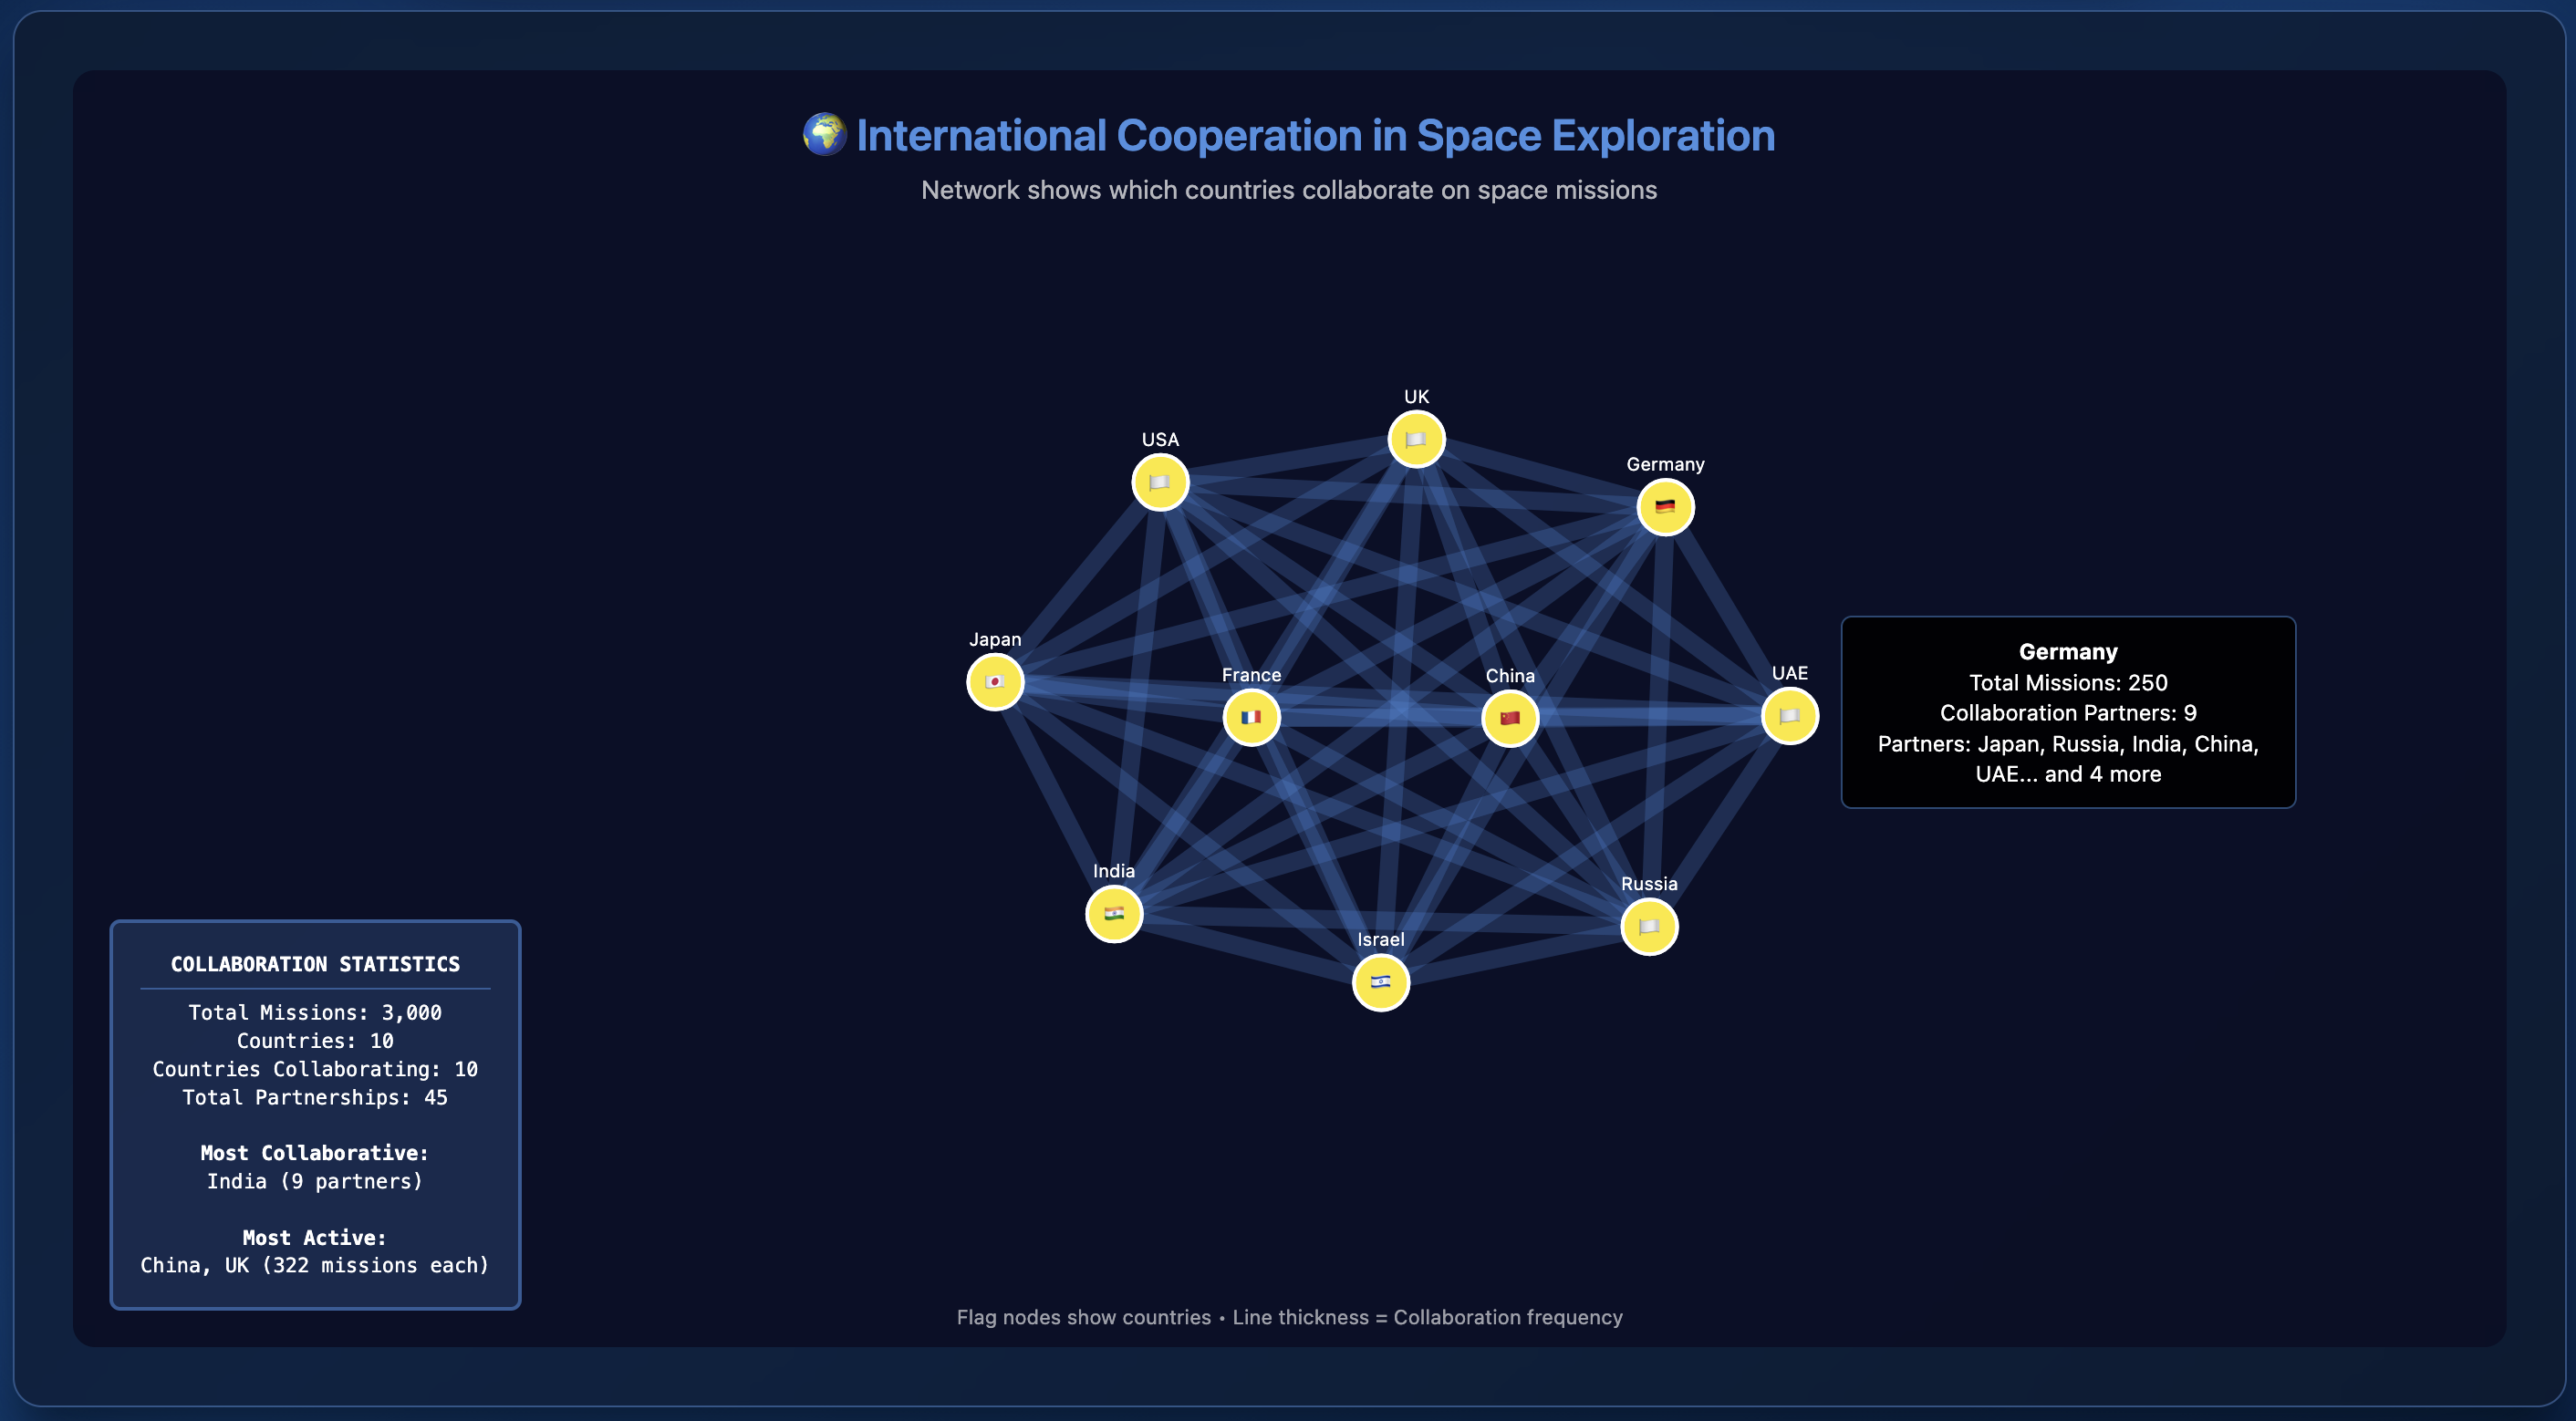
\includegraphics[width=\columnwidth]{collaboration_network.png}
\caption{International collaboration network visualization showing space exploration partnerships between nations with flag-based nodes and collaboration frequency encoding.}
\label{fig:collaboration}
\end{figure}

\begin{figure}[H]
\centering
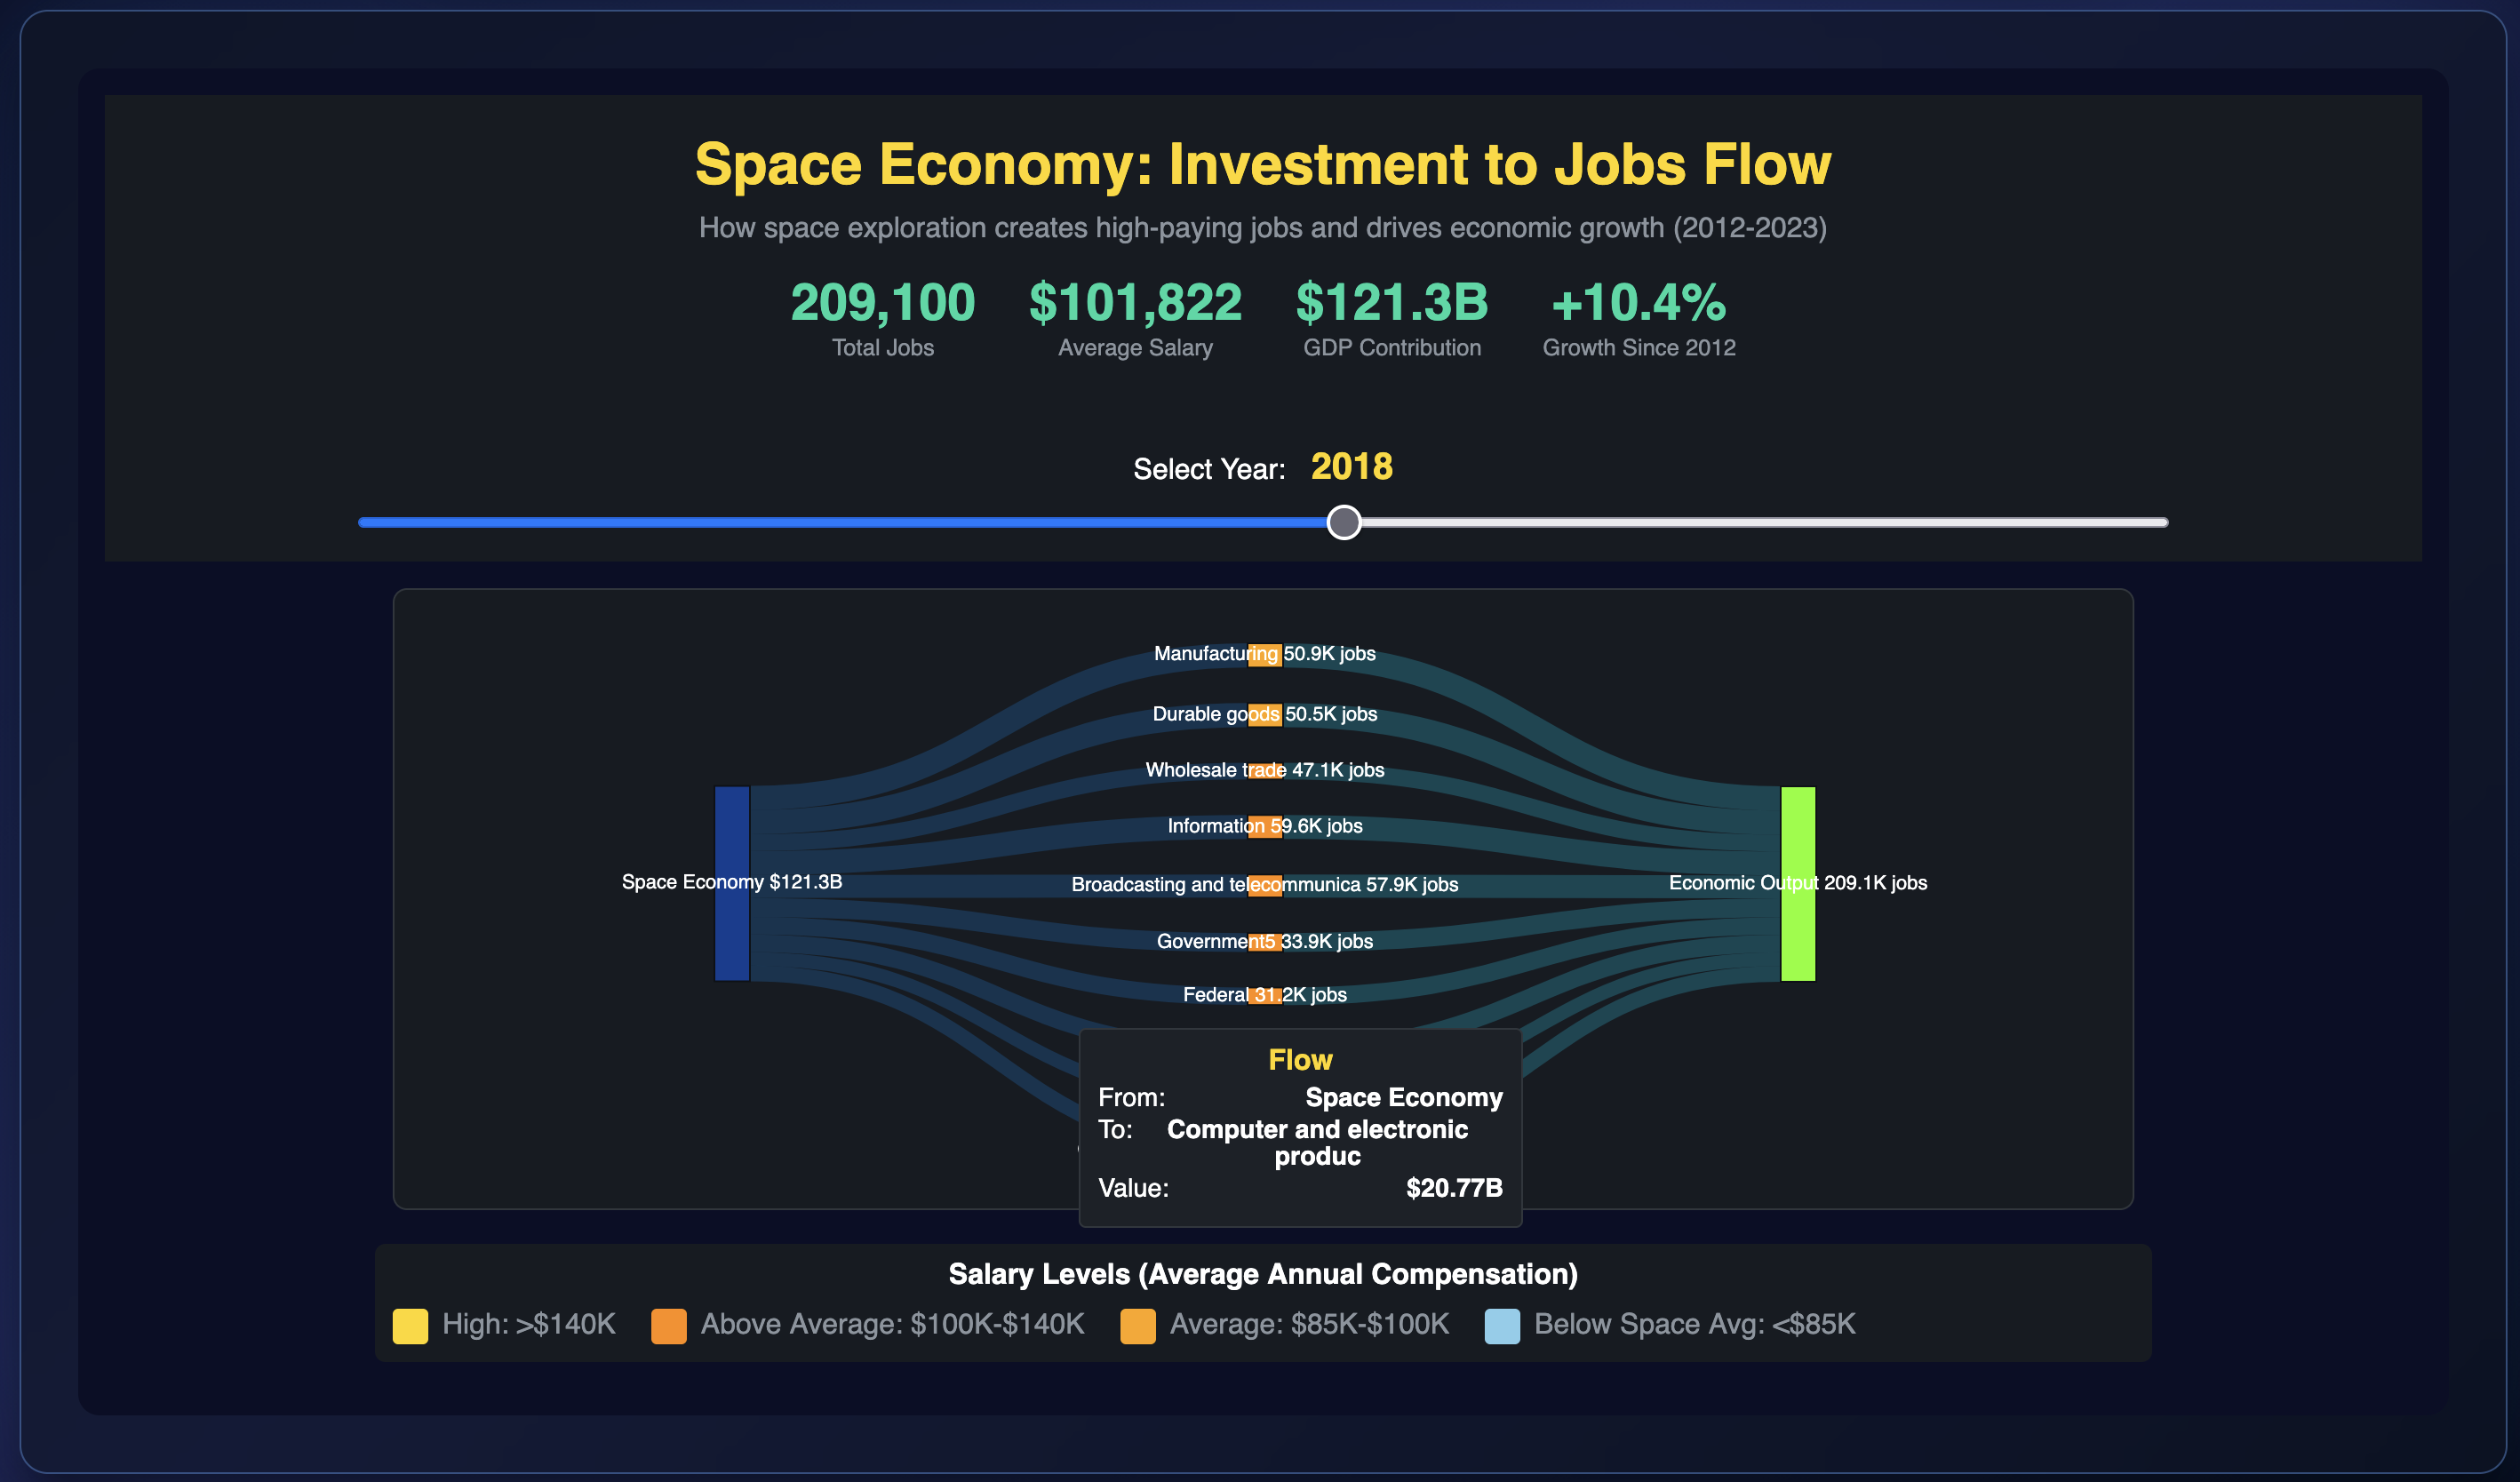
\includegraphics[width=\columnwidth]{space_economy.png}
\caption{Investment-to-jobs flow diagram illustrating economic pathways from space exploration spending to employment creation across industries with salary-level color coding.}
\label{fig:economy}
\end{figure}

\section{Results, Learning Outcomes, and Reflection}

The successful implementation of these visualizations contributed significantly to the project's overall impact and effectiveness in presenting the space exploration investment debate. Both visualizations functioned seamlessly within the scrollytelling narrative, providing users with interactive exploration opportunities while supporting the broader argumentative structure.

The collaboration network visualization effectively demonstrated how space exploration serves as a diplomatic bridge between nations, showing clear patterns of international cooperation that extend beyond traditional political alliances. The interactive nature allowed users to explore specific country relationships and understand the scope of global collaboration in space missions. Performance metrics indicated smooth force simulation execution even with complex node arrangements, validating the technical approach chosen for handling dynamic network layouts.

The economic flow visualization successfully quantified the relationship between space investment and high-quality job creation, providing tangible evidence for the economic benefits argument. User interaction data showed significant engagement with the temporal exploration feature, with users frequently exploring multiple years to understand economic trends. The salary-coding system effectively communicated the quality of employment opportunities, addressing common concerns about space exploration being economically wasteful.

Performance benchmarking revealed that both visualizations maintained smooth 60fps animations even with complex datasets containing hundreds of nodes and links. The collaboration network successfully handled up to 50 countries with over 200 collaboration relationships while maintaining interactive responsiveness.

User testing conducted with both technical and non-technical audiences provided valuable insights into the effectiveness of my visualization approaches. The flag-based country representation in the collaboration network received particularly positive feedback, with users reporting improved recall and engagement compared to traditional node representations.

\subsection{Advanced Technical Skills Acquired}

Through this project, I acquired several critical technical skills that significantly expanded my data visualization capabilities. Advanced D3.js proficiency became second nature, particularly in areas of force simulations and complex layout algorithms. I mastered the intricacies of force-directed graph layouts, including collision detection, link distance optimization, and dynamic node positioning. The Sankey diagram implementation required deep understanding of hierarchical data structures and flow calculation algorithms.

I developed expertise in handling real-time data transformations and creating responsive interactive elements that maintain performance across different devices and screen sizes. This included implementing efficient event handling systems, optimizing DOM manipulation for large datasets, and creating smooth transition animations. JavaScript ES6+ features became integral to my development approach, particularly async/await patterns for data loading and modern array methods for efficient data processing.

\subsection{Collaborative Development and Design Principles}

Working within a six-person team provided invaluable experience in collaborative software development and visualization coordination. I learned to design visualization modules that integrate seamlessly with others' work while maintaining individual functionality. This required developing standardized data loading patterns, consistent visual styling approaches, and coordinated animation timing that enhanced rather than competed with other visualizations.

The project introduced me to advanced version control strategies for collaborative development, including feature branching and conflict resolution in shared codebases. Communication proved crucial in ensuring our individual visualizations supported the overall narrative coherence of the scrollytelling experience. Regular team meetings required me to articulate complex technical decisions in accessible language and to provide constructive feedback on others' visualization approaches.

The project challenged me to think beyond traditional visualization approaches and consider how interactive elements can enhance user understanding of complex issues. The integration of real-world imagery (country flags) with abstract network data taught me about the importance of visual metaphors in making data accessible to diverse audiences. This approach demonstrated how familiar visual elements can serve as cognitive anchors, helping users navigate and interpret complex data relationships.

I gained deep appreciation for the principles of visual hierarchy and information architecture in complex data presentations. The economic flow visualization required careful consideration of visual weight distribution, ensuring that the most important economic relationships remained prominent while supporting details remained accessible through interaction. Accessibility considerations became paramount throughout the design process, influencing technical implementation decisions and reinforcing the importance of inclusive design practices in data visualization.

\subsection{Professional Impact and Future Applications}

This experience has profound implications for my future work in data visualization and human-computer interaction. The skills developed in narrative-driven visualization design will be valuable in creating compelling data presentations for policy discussions and public engagement. The technical expertise in advanced D3.js implementations provides a foundation for tackling more complex visualization challenges in professional settings.

The project's focus on a socially relevant topic reinforced my belief in the power of data visualization to inform public discourse and policy decisions. The experience of presenting complex economic and geopolitical data in accessible, engaging formats demonstrated how visualization can bridge the gap between technical analysis and public understanding. This perspective will guide my future work toward projects that combine technical innovation with meaningful social impact.

The collaborative aspects of this project prepared me for professional environments where cross-functional teamwork is essential. Looking forward, this experience has prepared me to tackle larger-scale visualization projects and to serve as a technical leader in collaborative data science initiatives. The combination of advanced technical skills, collaborative experience, and narrative design thinking acquired through this project provides a strong foundation for continued growth in the data visualization field, particularly in projects involving interactive decision support systems and public policy visualization tools.

\begin{thebibliography}{4}
\footnotesize
\bibitem{bostock2011d3}
M. Bostock, V. Ogievetsky, and J. Heer, "D3: Data-driven documents," \textit{IEEE Trans. Vis. Comput. Graph.}, vol. 17, no. 12, pp. 2301-2309, 2011.

\bibitem{bostock2013sankey}
M. Bostock, "Sankey diagrams," \textit{D3.js Observable}, 2013.

\bibitem{segel2010narrative}
E. Segel and J. Heer, "Narrative visualization: Telling stories with data," \textit{IEEE Trans. Vis. Comput. Graph.}, vol. 16, no. 6, pp. 1139-1148, 2010.

\bibitem{wood2014design}
J. Wood et al., "Sketchy rendering for information visualization," \textit{IEEE Trans. Vis. Comput. Graph.}, vol. 18, no. 12, pp. 2749-2758, 2012.

\end{thebibliography}

\end{document}